\section{Experimental Evaluation}
\label{sec:experiments}

\subsection{Benchmarks and Execution Checks}
\label{sec:setup}

The benchmarks in Table~\ref{tab:measured_design} work backward from observed prices. The intraday runs (RQ1) measure when trades occur and both sides of the book are present under matched randomness. The shared-parent branches (RQ2) then track how a common infection event changes social states and how behavioral and regulatory interventions affect orders and fills. The fixed-observation and schedule benchmarks (RQ3) move upstream to compare intents across decision backends and identify which scheduled requests could carry a public announcement. Rule-world profiles measure the cost of retaining and verifying the state history that makes these paths auditable.

\begin{table*}[t]
  \centering\small
  \caption{\tr{实测基准及离线调度核对的配置。长周期参考配置见附录~\ref{app:benchmark_details_zh}。}{Settings for the Measured Benchmarks and Offline Schedule Audit. Appendix~\ref{app:benchmark_details} gives the prospective long-horizon configuration.}}
  \label{tab:measured_design}
  \begin{tabularx}{\textwidth}{@{}p{0.24\textwidth} p{0.28\textwidth} X@{}}
    \toprule
    \tr{评估任务}{Evaluation} & \tr{执行配置}{Settings} & \tr{比较单位}{Unit of comparison} \\
    \midrule
    \tr{日内交易活动（RQ1）}{Intraday activity (RQ1)} &
    $N=100$, $T=T_{\rm day}=100$, $p_{\rm act}=0.05$ &
    \tr{三个匹配种子，各比较三种规则策略。}{Three matched seeds, each shared by three rule policies.} \\
    \tr{共同父世界分支（RQ2）}{Shared-parent branches (RQ2)} &
    $N=20$, $T_{\rm day}=4$, $p_{\rm act}=1$, \tr{27 步事件窗}{27 event steps} &
    \tr{一个父世界，十一条分支。}{Eleven branches from one parent world.} \\
    \tr{固定观察（RQ3）}{Fixed observations (RQ3)} &
    \tr{九类画像 $\times$ 三类对比 $\times$ 两个状态}{Nine archetypes $\times$ three contrasts $\times$ two states} &
    \tr{54 次真实 LLM 请求，构成 27 对比较。}{54 live LLM requests, organized into 27 pairs.} \\
    \tr{离线调度核对（RQ3）}{Offline scheduling (RQ3)} &
    $N=100$, $p_{\rm act}=0.05$, $k=10$, $T_{\rm slow}=10$ &
    \tr{20 个固定种子在公告发布步的计划资格。}{Scheduled eligibility at announcement release across 20 fixed seeds.} \\
    \tr{规则运行剖面（RQ3）}{Rule profiles (RQ3)} &
    \tr{同一平台 $N=100$、$T=100,200$；另一平台 $N=1{,}000$、$T=12$}{Same host $N=100$, $T=100,200$; second host $N=1{,}000$, $T=12$} &
    \tr{Mac 各期限一次完整剖面；ASUS 保存 12 步、终期剖面未完成。}{One complete Mac profile per horizon. The ASUS run saved 12 steps and stopped during final profiling.} \\
    \bottomrule
  \end{tabularx}
\end{table*}


The three rule policies use seeds 932201--932203. Across all 900 committed steps, the cash, share, and fee residuals are zero. Read-only restoration on the same platform matches the terminal state hash in all nine trajectories (Table~\ref{tab:invariants}). Each seed is the unit of comparison across policies.

\subsection{Market Activity and Quote Coverage (RQ1)}
\label{sec:exp:rq1}

We hold the activity mask, lognormal quote shocks, resource constraints, and matching rules fixed within each seed. Zero-intelligence agents draw buy and sell actions with symmetric probabilities and can hold~\cite{gode1993allocative}. The homogeneous linear-value policy retains acquisition cost and the recent high as anchors. Its valuation is linear, its risk tolerance is fixed at 0.5, and its order policy excludes social and loss feedback.

\begin{figure*}[t]
 \centering
 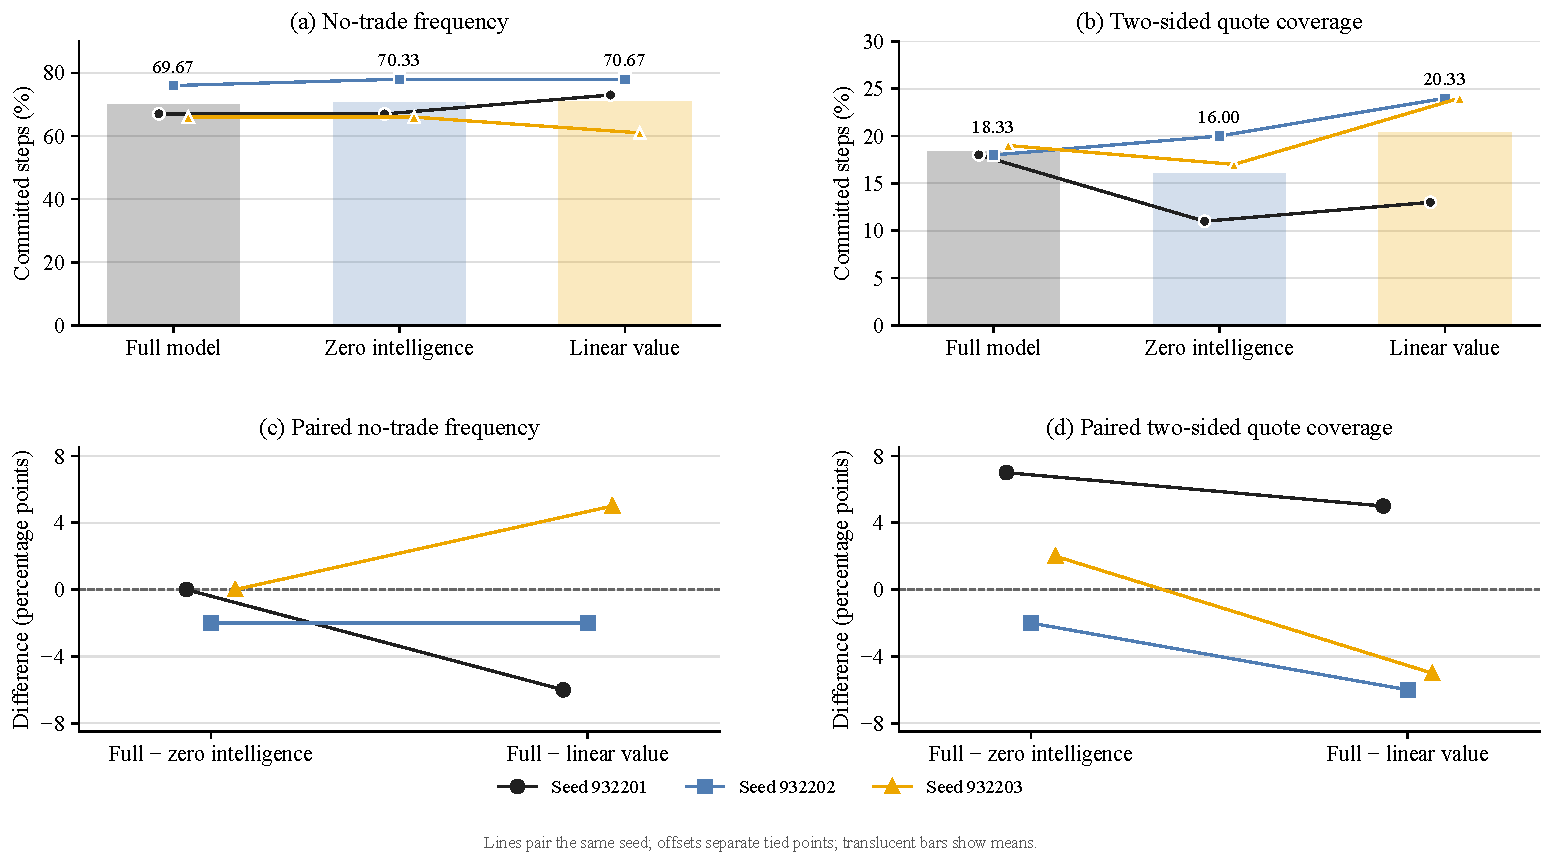
\includegraphics[width=0.96\textwidth]{figures/fig2_rq1_stylized_facts.pdf}
 \caption{Intraday activity in nine rule trajectories. The upper panels show the percentage of steps without trades and the percentage with two-sided quotes. The lower panels show the full model minus each baseline within the same seed, in percentage points. Bars in the upper panels denote means, with matched trajectories linked across policies. Small horizontal offsets distinguish overlapping markers.}
 \Description{Two panels of activity and quote coverage by policy and two panels of matched-seed differences.}
 \label{fig:rq1}
\end{figure*}

\paragraph{Quote coverage varies across matched seeds.}
With an activation probability of 0.05 and a one-step order lifetime, 61--78\% of steps have no fills and 11--24\% have quotes on both sides. The full model averages 69.67\% of steps without trades and 18.33\% with two-sided quotes. The corresponding figures are 70.33\% and 16.00\% for zero intelligence and 70.67\% and 20.33\% for linear value. The full-minus-baseline coverage differences are $+7,-2,+2$ percentage points against zero intelligence and $+5,-6,-5$ against linear value. The ranking changes across the three blocks (Figure~\ref{fig:rq1}, Table~\ref{tab:rq1_results}).

The quoted spread $10^4(P^{\rm ask}-P^{\rm bid})/P^{\rm mid}$ is conditional on both queues being present at a tradable step. Reporting quote coverage alongside the spread makes its sampling denominator explicit. Each trajectory spans one model trading day. The corresponding multi-day protocol uses daily log returns $r_d=\log(P_d/P_{d-1})$ to evaluate excess kurtosis, return and absolute-return autocorrelations, and the correlation of volume with $|r_d|$~\cite{cont2001empirical} (Appendix~\ref{app:benchmark_details}).

\subsection{Feedback Across Scales (RQ2)}
\label{sec:exp:rq2}

\begin{figure*}[t]
 \centering
 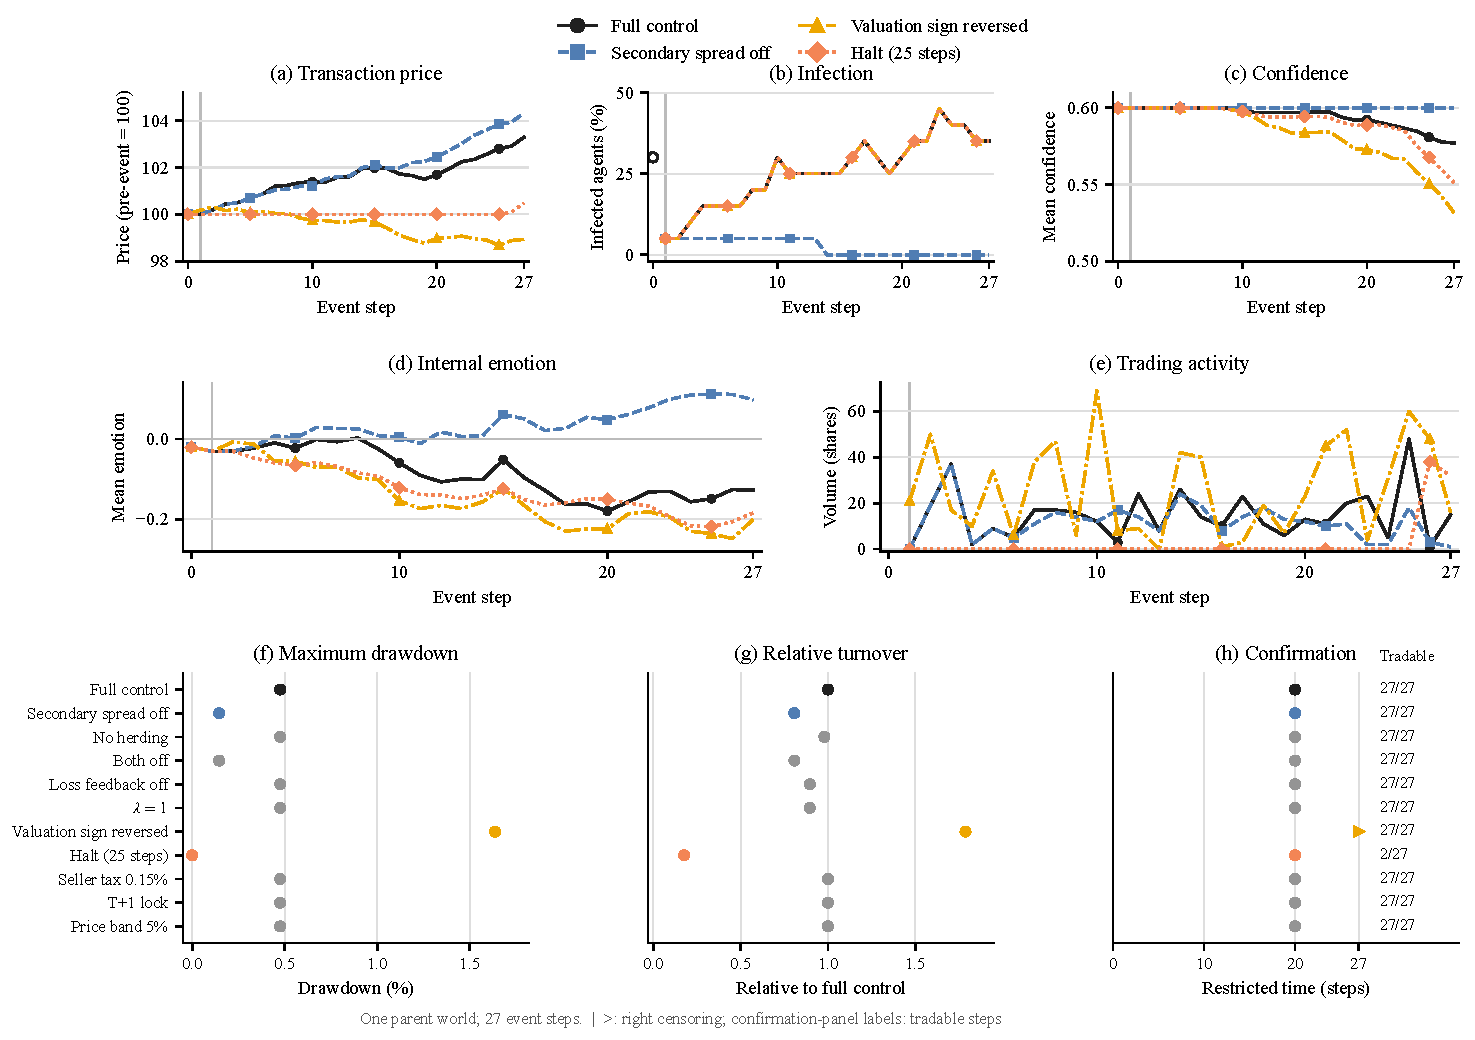
\includegraphics[width=\textwidth]{figures/fig3_rq2_mechanisms_policy.pdf}
 \caption{Social, behavioral, and market responses in one shared parent world. The time-series panels align infection, population means of model confidence and sentiment, indexed price, and share volume on the same event clock. The open marker in panel (b) denotes the pre-event checkpoint (6 of 20 infected). At $u=1$, the common event resets all SIRS states to susceptible and seeds one infection (1 of 20). The outcomes below show all eleven branches. The arrowhead marks right censoring at $u=27$.}
 \Description{Five aligned event-time series and three outcome plots for drawdown, turnover, and price confirmation.}
 \label{fig:rq2}
\end{figure*}

\paragraph{Shared-checkpoint design.}
All branches begin at the fifth commit of seed 933001, with 20 investors, four steps per day, and every investor active at each event step. Six investors are already infected at the common checkpoint $u=0$. At $u=1$ (tick 6), the event sets all investors to susceptible and directly infects one investor. The 30\% checkpoint prevalence and the 5\% prevalence at the first event commit therefore describe the states before and after this common reinitialization. The branches share the random streams for 27 event steps. We record infection, population mean confidence and sentiment, the last-trade price, and traded share volume at each commit (Figure~\ref{fig:rq2}).

Maximum drawdown is the largest decline from a running peak initialized at the pre-event price. Relative turnover divides each branch's traded share volume by that of the full control. The price-confirmation rule records the step completing 20 consecutive prices at or above 98\% of the pre-event price after the first global trough, which can be $u=0$. Unconfirmed times are right-censored at the window boundary (Table~\ref{tab:rq2_results}).

\paragraph{Social dynamics and market responses.}
In the full control, infection peaks at 45\% at $u=23$ (Figure~\ref{fig:rq2}b). Mean confidence begins to fall at $u=10$ and reaches 0.577 at the end of the window. Mean internal emotion reaches $-0.180$ at $u=20$ (panels c--d). Suppressing secondary contagion confines infection to the seeded investor until it clears at $u=14$. In that branch, confidence stays near 0.600 and mean emotion reaches $+0.112$ at $u=25$. Suppressing spread also reduces volume from 395 to 319 shares (panel e) and raises the final price index from 103.28 to 104.31 (panel a). Maximum drawdown falls from 0.4754\% to 0.1453\%, a reduction of 0.3301 percentage points (69.4\% relative).

Disabling confidence-dependent herding leaves peak infection at 45\%. Prices in the two branches coincide through $u=22$, including the local peak at $u=15$ and trough at $u=19$ that determine the 0.4754\% maximum drawdown. Volume already differs by one share at that trough, and total volume falls from 395 to 387 shares (relative turnover 0.9797). With $Y$ denoting drawdown and binary indices denoting contagion and herding, the four-branch interaction $Y_{11}-Y_{10}-Y_{01}+Y_{00}$ is zero in this world.

\paragraph{The sign of retrospective valuation changes the price response.}
The infection event changes the social state, and prices respond to the resulting orders and fills. In Equation~\eqref{eq:aggregate_v}, a price above a retrospective reference adds a positive term to the valuation and can raise the buying propensity when the other inputs are held fixed. The aggregate order direction also depends on the remaining references, sentiment, and risk. Reversing the retrospective signs lowers the final price to 1.07\% below the pre-event price, raises maximum drawdown to 1.6372\%, and raises relative turnover to 1.7873. The branch with $\lambda=1$ and the branch that also removes dynamic loss feedback both record 0.4759\% drawdown and 0.8962 relative turnover.

\paragraph{Trading rules affect different parts of the exchange.}
A 25-step halt leaves two tradable steps and a relative turnover of 0.1772. Drawdown is zero. The book is cleared at the start of the halt. The price carries forward for 25 steps with zero fills. During that interval, infection peaks at 45\%, and mean internal emotion reaches $-0.218$ at $u=25$. At $u=26$, 38 shares trade as matching resumes (Figure~\ref{fig:rq2}a--e). The other three policy branches retain all 27 tradable steps and produce the same 87 fills as the control. In the 5\% band branch, submitted and executed prices deviate at most 1.092\% from their contemporaneous daily anchors. The $T+1$ rule locks up to 72 shares and leaves the realized sell orders and fills unchanged. The 0.15\% seller tax changes the settlement debit directly, leaving share sizing in Equation~\eqref{eq:order_quantity} unchanged at a given state. In this window the tax receipts rise from 20.286250 to 60.858750 currency units, with the same fills.

\paragraph{The confirmation floor reflects the short event window.}
The first trough is the pre-event price in ten branches, all of which reach the earliest confirmation at step 20. The halted branch reaches that threshold using carried-forward prices during the suspension. The reversed-valuation branch reaches its first trough at step 25 and has two subsequent observations, leaving its time right-censored at 27. The series remain above the 98\% threshold throughout this parent-world comparison. Here the confirmation measure records elapsed observations after the trough. Tradable steps and turnover give it an economic interpretation.

\subsection{Decision Interfaces and Computational Cost (RQ3)}
\label{sec:exp:rq3}

\begin{figure*}[t]
 \centering
 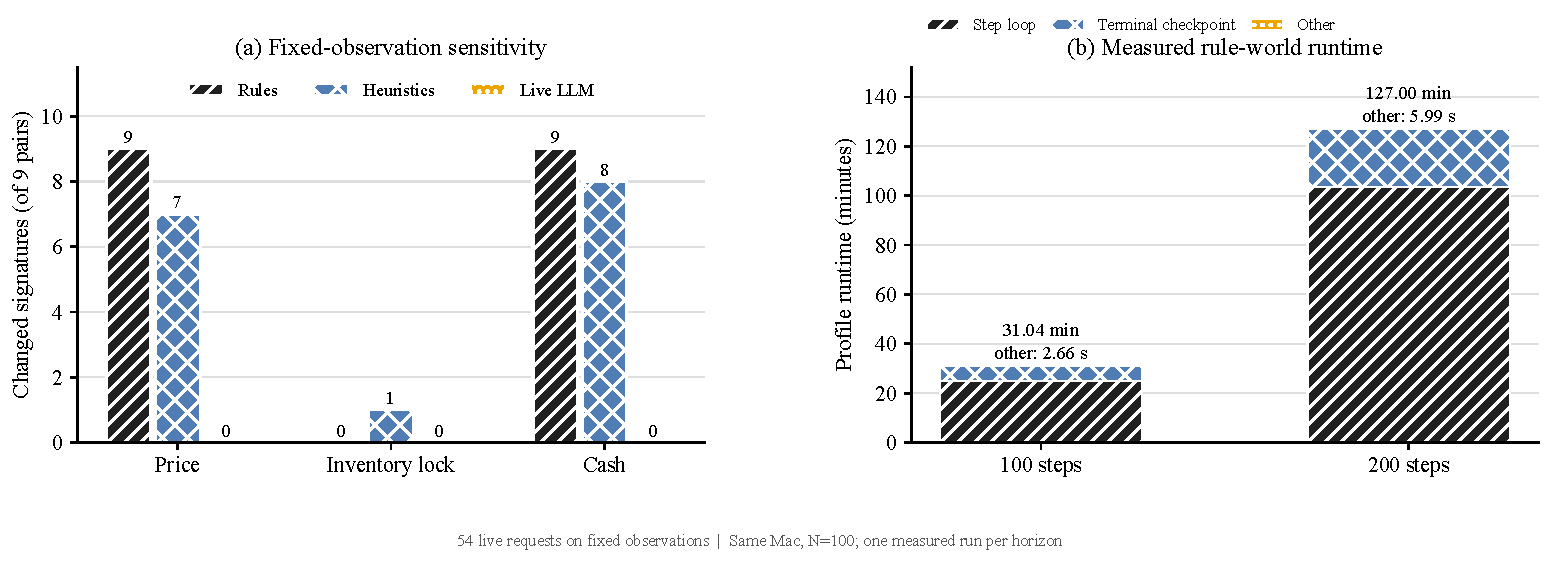
\includegraphics[width=\textwidth]{figures/fig4_rq3_cognition_cost.pdf}
 \caption{Fixed-observation responses and rule-world runtime. The response panel counts changes in economic action signatures across nine pairs per contrast. The runtime panel separates the durable step loop, terminal checkpoint, and remaining profile time for two $N=100$ runs on the same machine.}
 \Description{Action changes for price, inventory lock, and cash contrasts, and stacked profile times at two horizons.}
 \label{fig:rq3}
\end{figure*}

\paragraph{The fixed-observation benchmark exercises the decision contract.}
Nine archetypes, three contrasts (price, locked inventory, cash), and two states per contrast give 54 request cells, 45 distinct constructed observations, and 27 pairs. We use neutral wording, temperature zero, and a 2,048-token output limit. The request configuration and archived OpenAI API responses identify the model by the alias \texttt{gpt-6-luna}.

An economic action signature records direction, signed share quantity, and limit price. It changes in 18/27 rule pairs, 16/27 heuristic pairs, and 0/27 LLM pairs (Figure~\ref{fig:rq3}a and Table~\ref{tab:pilot}). Rules return 45 buys and nine holds. The LLM requests serialize both the constructed current state and the template behavioral trace stored in the private \texttt{behavior} field. The risk and price-reference values differ between these records in all 54 requests. Every model response is \texttt{HOLD} and passes the schema, protocol identity, evidence-ID, and resource checks. The evidence-ID check verifies that cited IDs are distinct members of the visible set. The signature contrast characterizes the backends on these constructed inputs. An additional comparison with aligned state and trace fields would be needed to isolate the effect of the discrepancy.

\paragraph{Archetype-specific order changes.}
Under numerical rules, the price contrast changes signed quantity by $-2$ shares for every archetype, and the cash contrast changes it by $-12$ shares (Figure~\ref{fig:persona_deltas}). Under persona heuristics, the price contrast shifts the arbitrageur and stabilization fund by $-102$ and $-63$ shares, respectively. The insurer changes from a 10-share sell order to \texttt{HOLD} in the inventory-lock contrast. In the separate price contrast, the insurer retains the same signed quantity and raises its limit by 1,002 ticks, the dagger-marked cell.

\begin{figure*}[t]
 \centering
 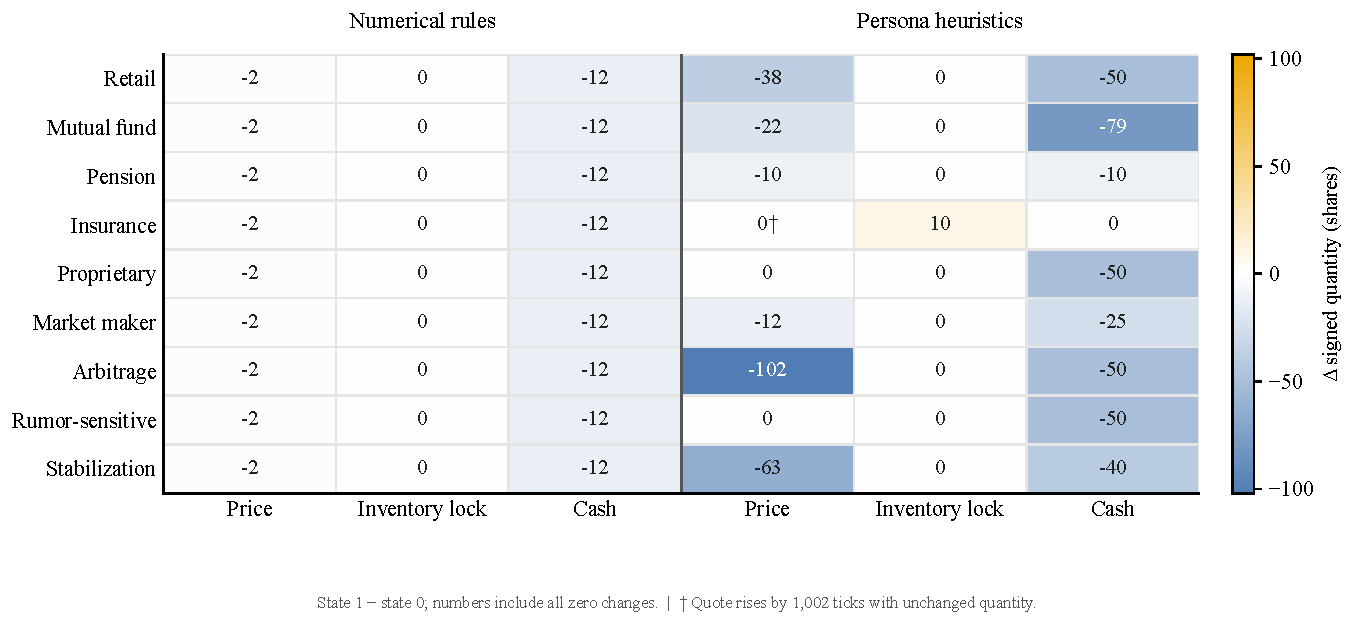
\includegraphics[width=0.96\textwidth]{figures/archetype_order_response.pdf}
 \caption{Changes in signed order size across nine archetypes. Each cell gives the perturbed minus baseline share quantity for one contrast and backend. A buy has positive sign, a sell negative sign, and a hold zero quantity. A dagger marks a price change with unchanged quantity.}
 \Description{Nine rows of archetypes and six columns of signed order size changes for the rule and heuristic backends.}
 \label{fig:persona_deltas}
\end{figure*}

\paragraph{Request accounting and scheduled event access.}
The live batch uses 119,637 input and 9,306 output tokens in 69.597 seconds. Median request latency is 2.297 seconds. Logged usage and frozen rates give an accounted cost upper bound of USD 0.03456225 (Table~\ref{tab:rq3_results}). An offline check separately intersects the activation masks and request schedules at the announcement step. For 20 fixed seeds, the announcement coincides with a periodic request step. Full scheduling offers 101 eligible requests across all seeds. The periodic slow group offers one request in each of ten seeds. In the other ten, no slow-group agent is active at release (right panel of Figure~\ref{fig:schedule_exposure}). Equation~\eqref{eq:cost_ratio} gives the expected request fraction across a full horizon. The release-step counts show how the same schedule affects access to a specific announcement.

\paragraph{Cumulative recording drives a term in the runtime cost.}
Extending the same-seed, 100-agent rule world from 100 to 200 steps on an Apple M5 (24 GiB) increases the profiled time from 1,862.397 to 7,619.767 seconds, a factor of 4.091. Peak process memory increases from 1.239 to 2.486 GiB. The terminal checkpoint, which includes reconstruction from persisted deltas, takes 364.780 and 1,394.507 seconds. Execution, commit, durable publication, and the terminal checkpoint together account for 89.9\% and 91.0\% of the two profiles. The decision phase takes 2.895 and 5.789 seconds.

The archival implementation repeatedly validates, copies, and hashes growing histories of decisions, receipts, and ledger entries. When retained history grows linearly in $t$, a full scan per step contributes $\sum_{t=1}^{T}\mathcal{O}(t)=\mathcal{O}(T^2)$ at fixed population. This term describes the work of processing cumulative history. Figure~\ref{fig:rq3} shows the two measured profiles of the full runner. On the AMD Ryzen AI 7 H 350 platform, the 1,000-agent run saves all 12 steps and reaches a sampled memory peak of 1.692 GiB before the controller stops during final profiling. In three timing repeats of the same 100-agent, 12-step world, scalar-optimized strict validation reduces total time by 1.52--3.08\% (Figure~\ref{fig:timing_supp}).
